\section{附录}
    \subsection{指令系统}
    \begin{figure}[!hbp]
            \centering
            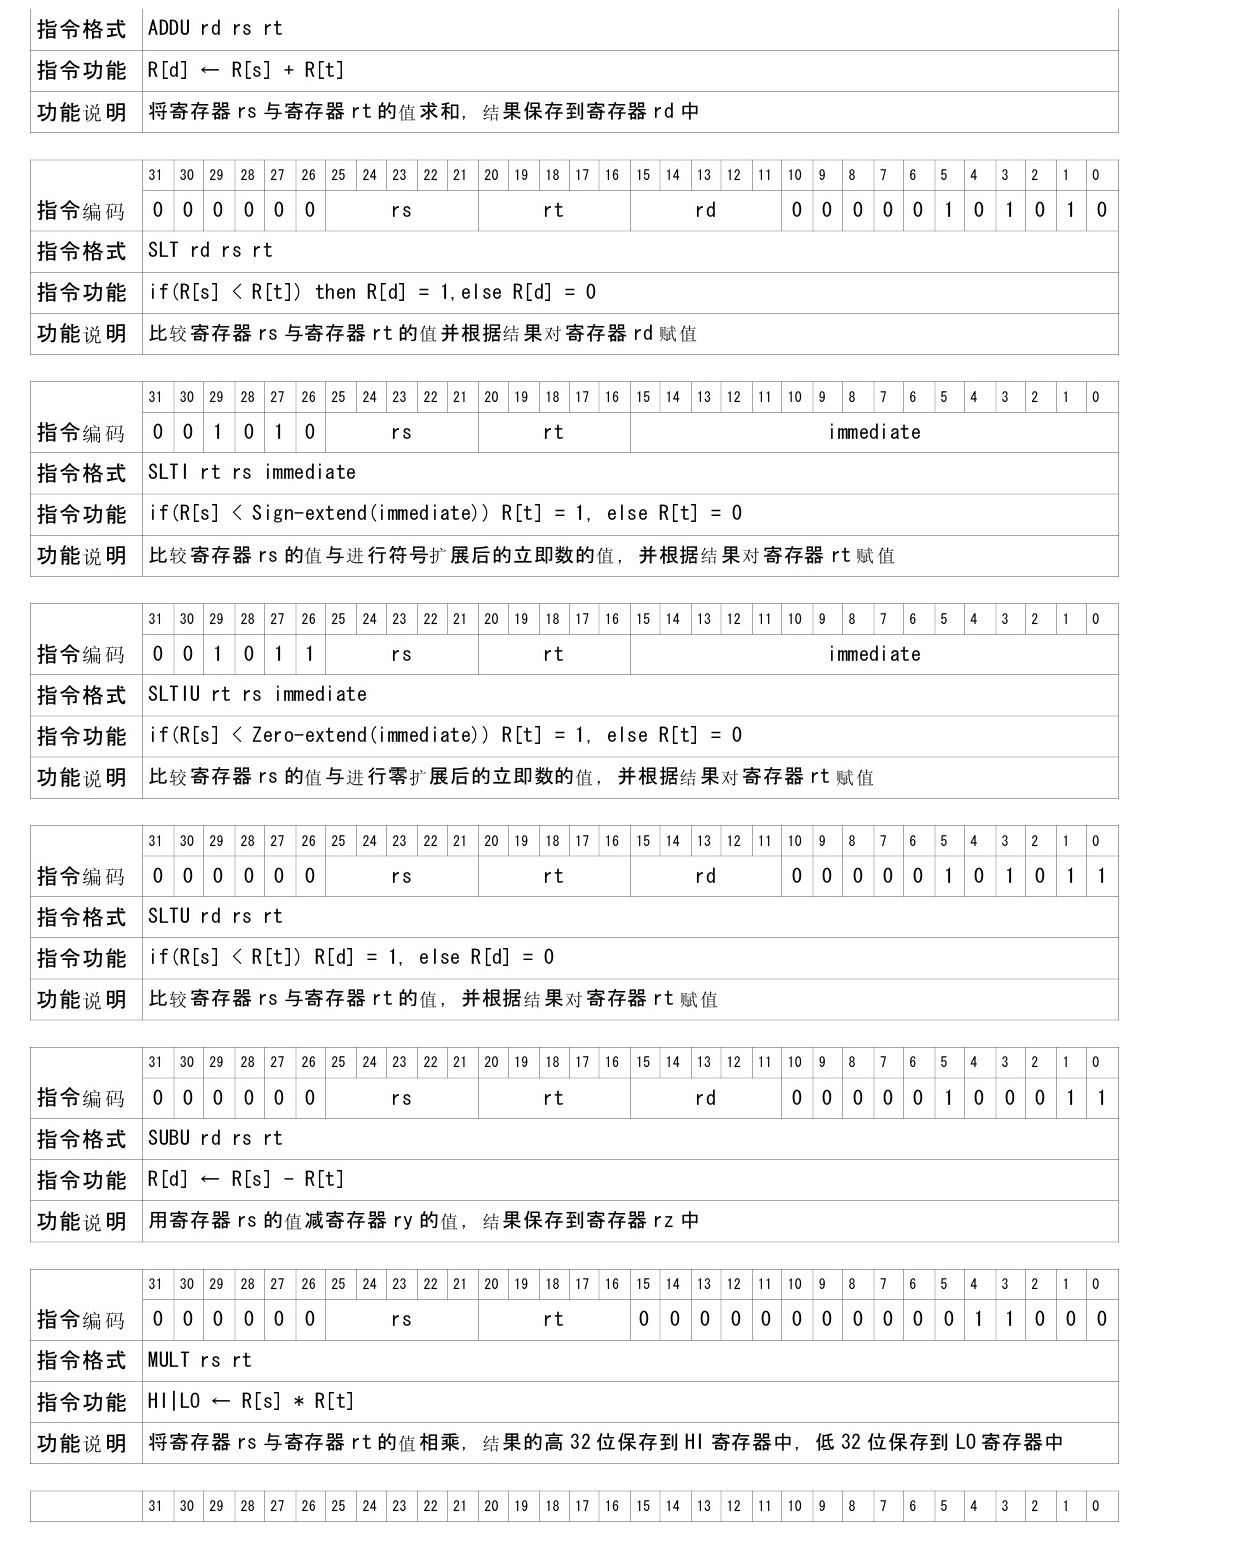
\includegraphics[width=\textwidth]{chart/insert1.jpg}
    \end{figure}
    
    \begin{figure}[!hbp]
            \centering
            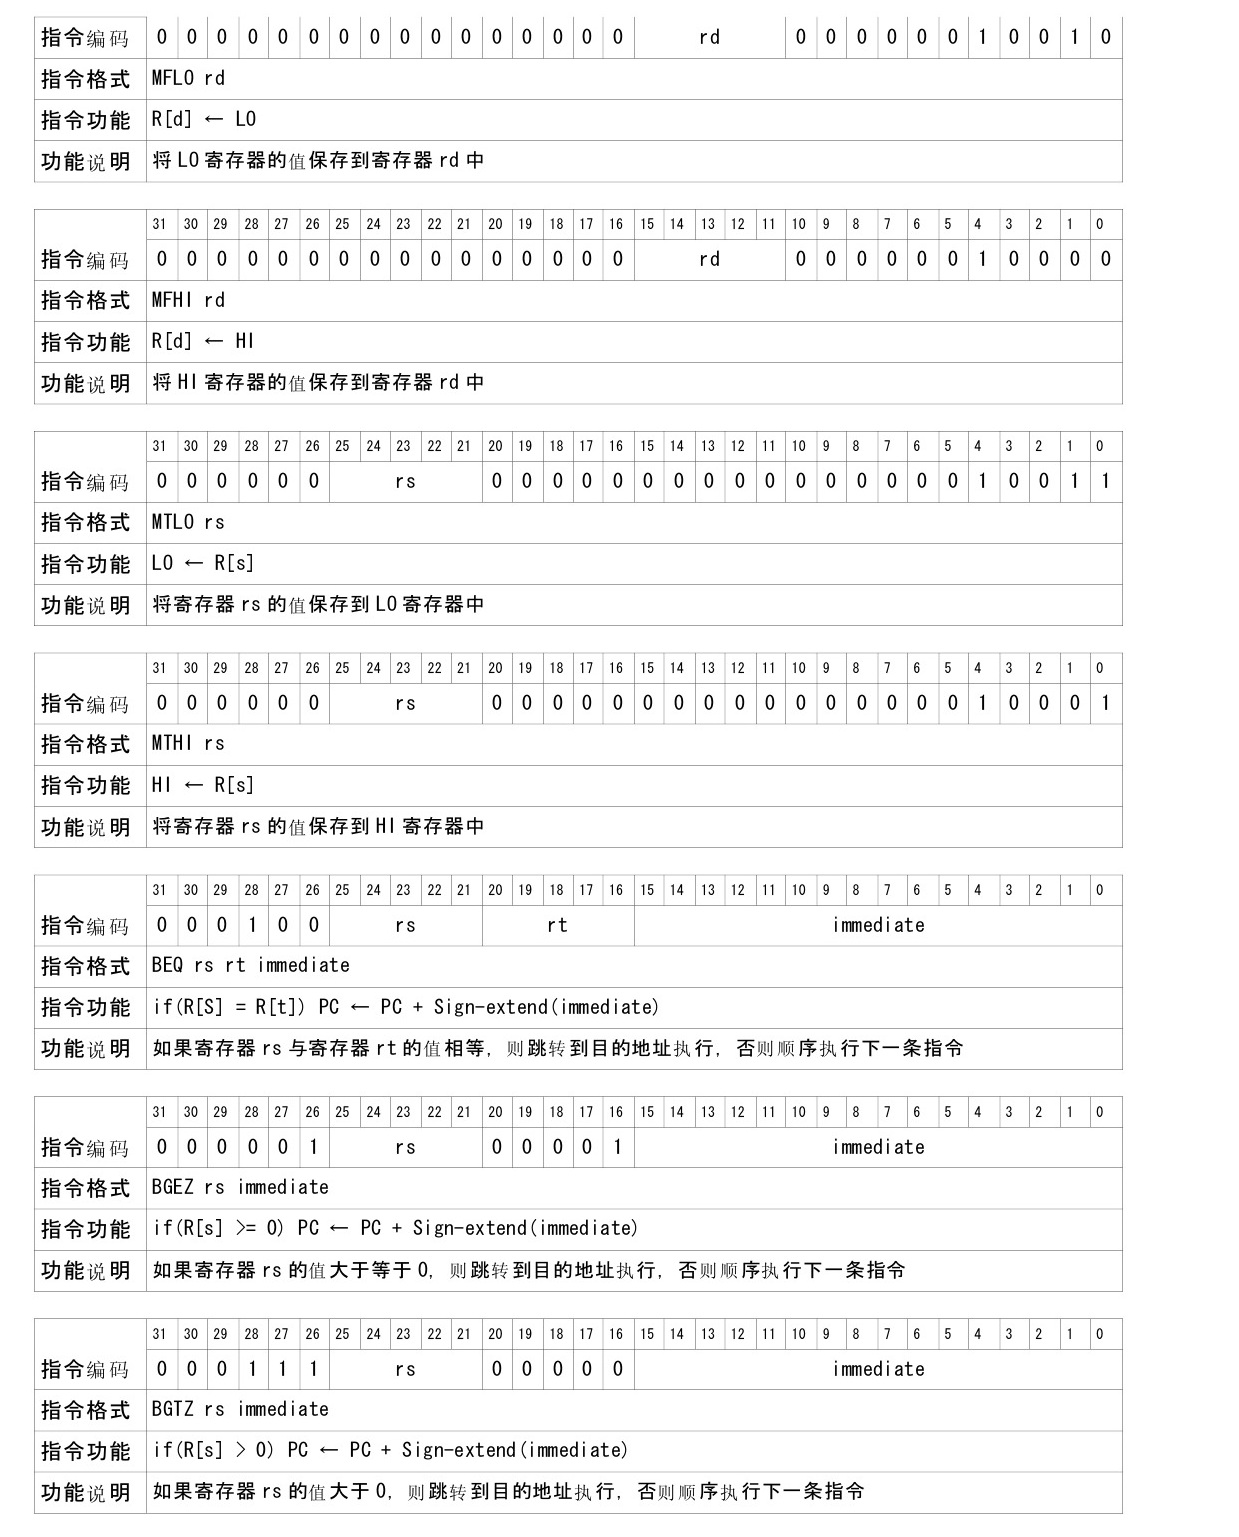
\includegraphics[width=\textwidth]{chart/insert2.jpg}
    \end{figure}
    
    \begin{figure}[!hbp]
            \centering
            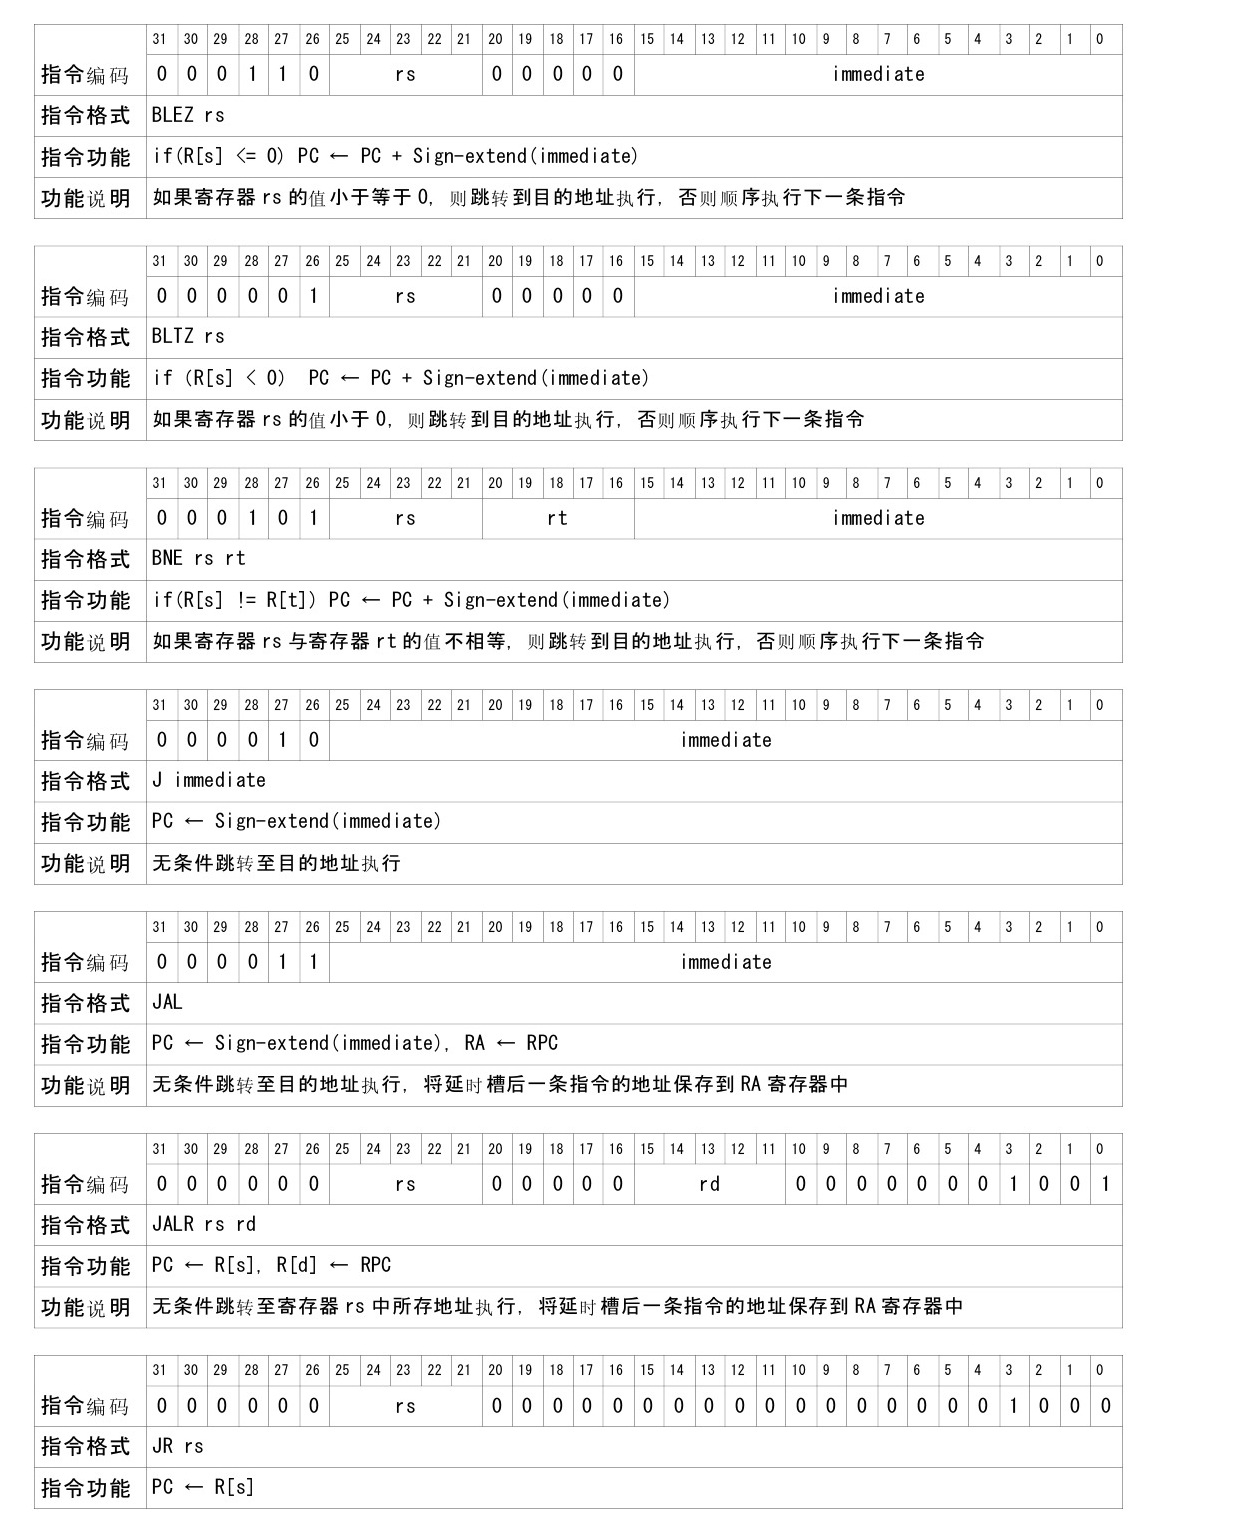
\includegraphics[width=\textwidth]{chart/insert3.jpg}
    \end{figure}

    \begin{figure}[!hbp]
            \centering
            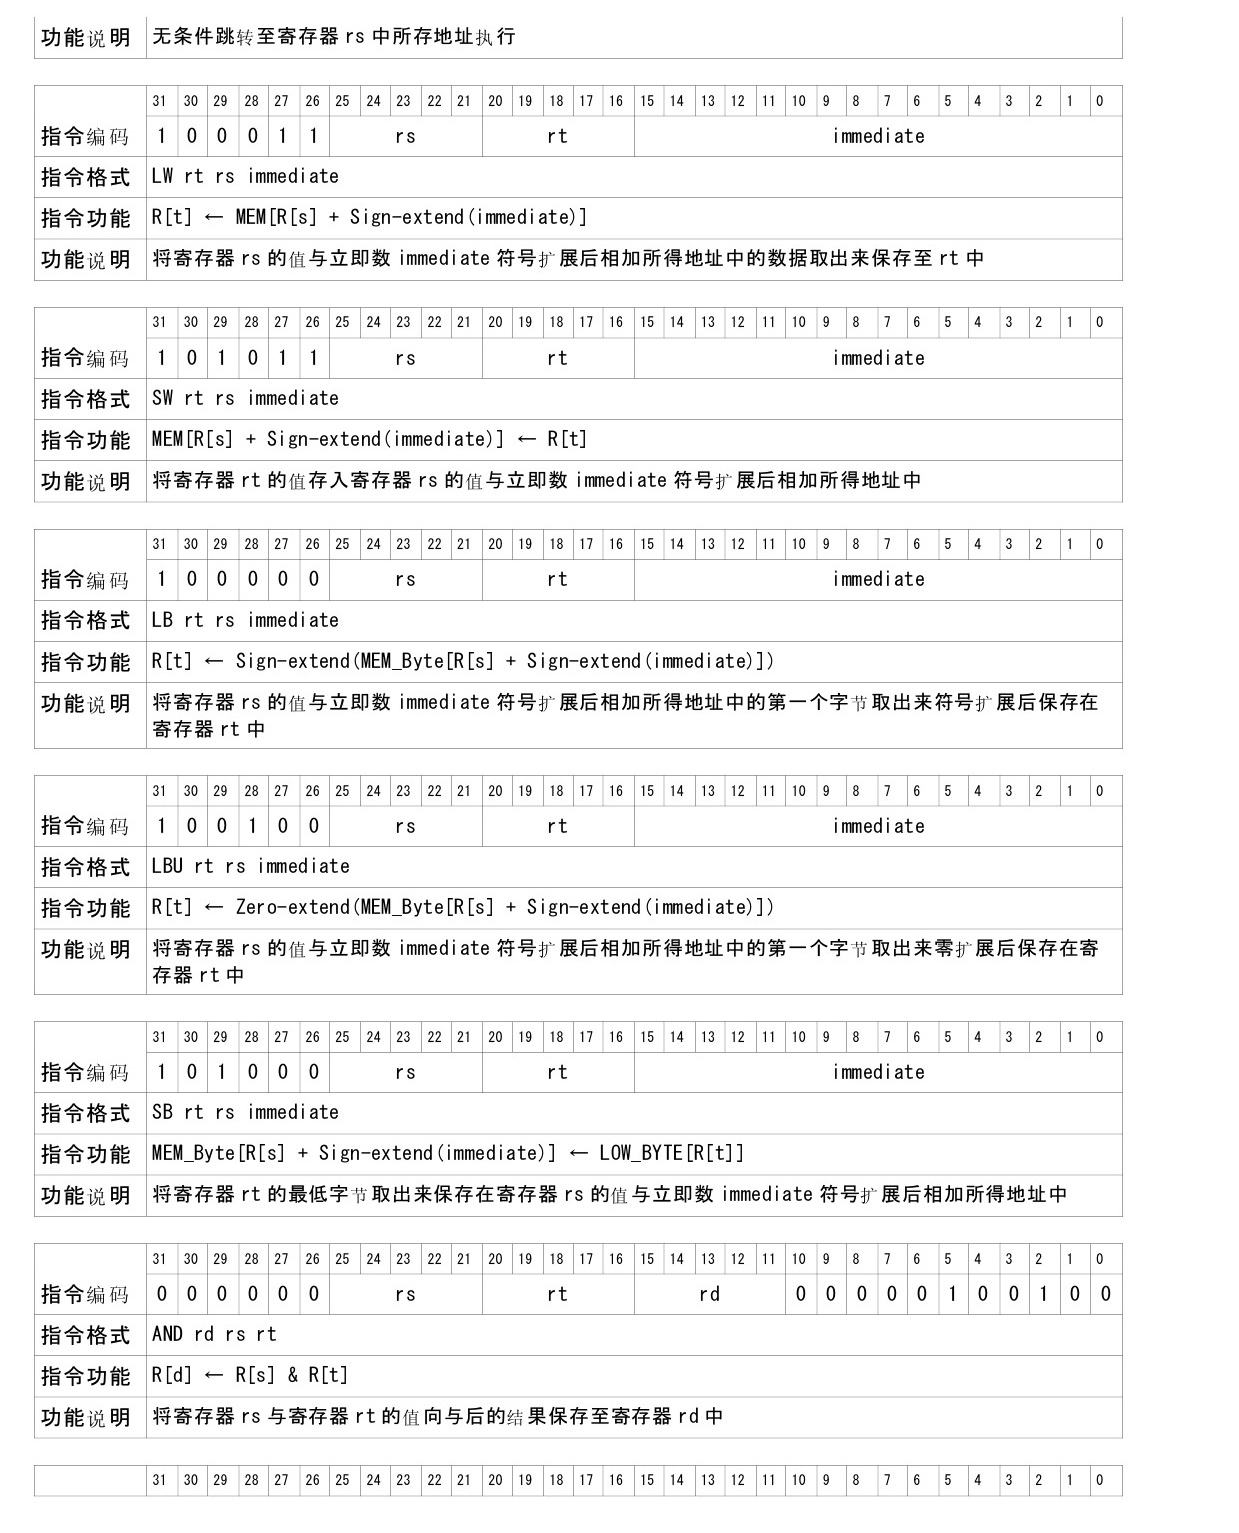
\includegraphics[width=\textwidth]{chart/insert4.jpg}
    \end{figure}

    \begin{figure}[!hbp]
            \centering
            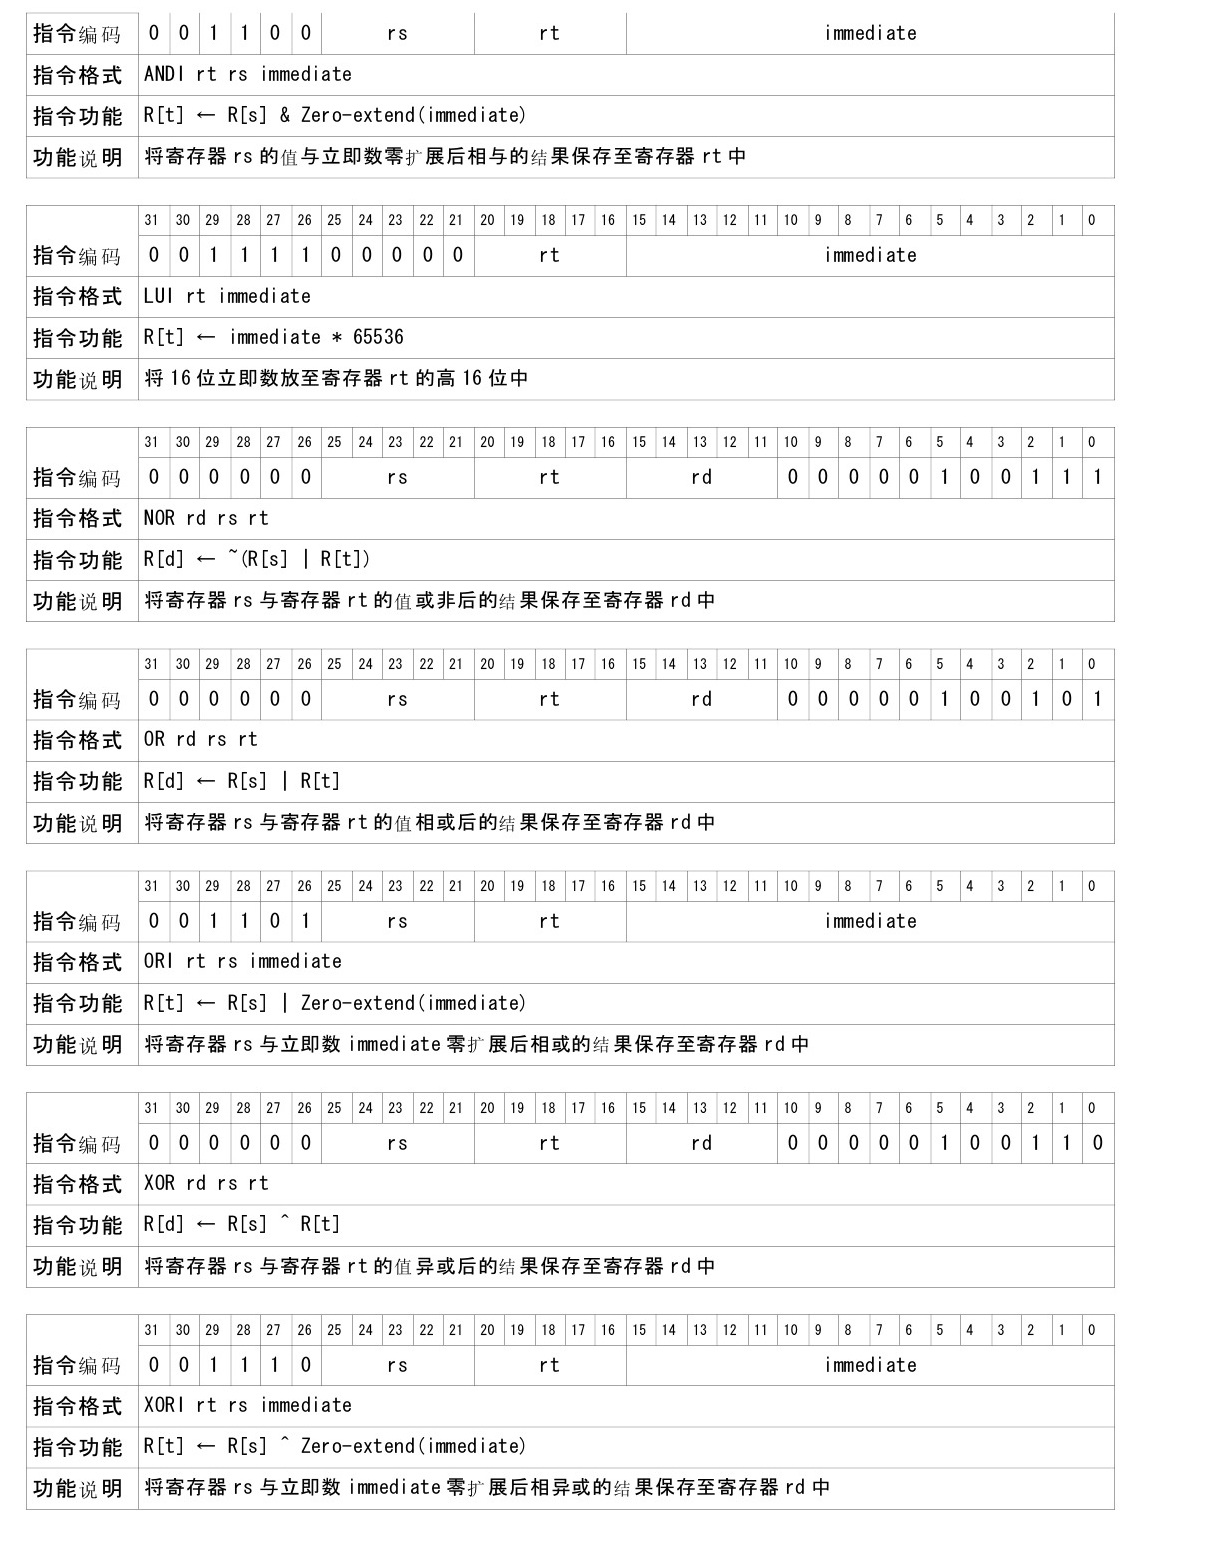
\includegraphics[width=\textwidth]{chart/insert5.jpg}
    \end{figure}

    \begin{figure}[!hbp]
            \centering
            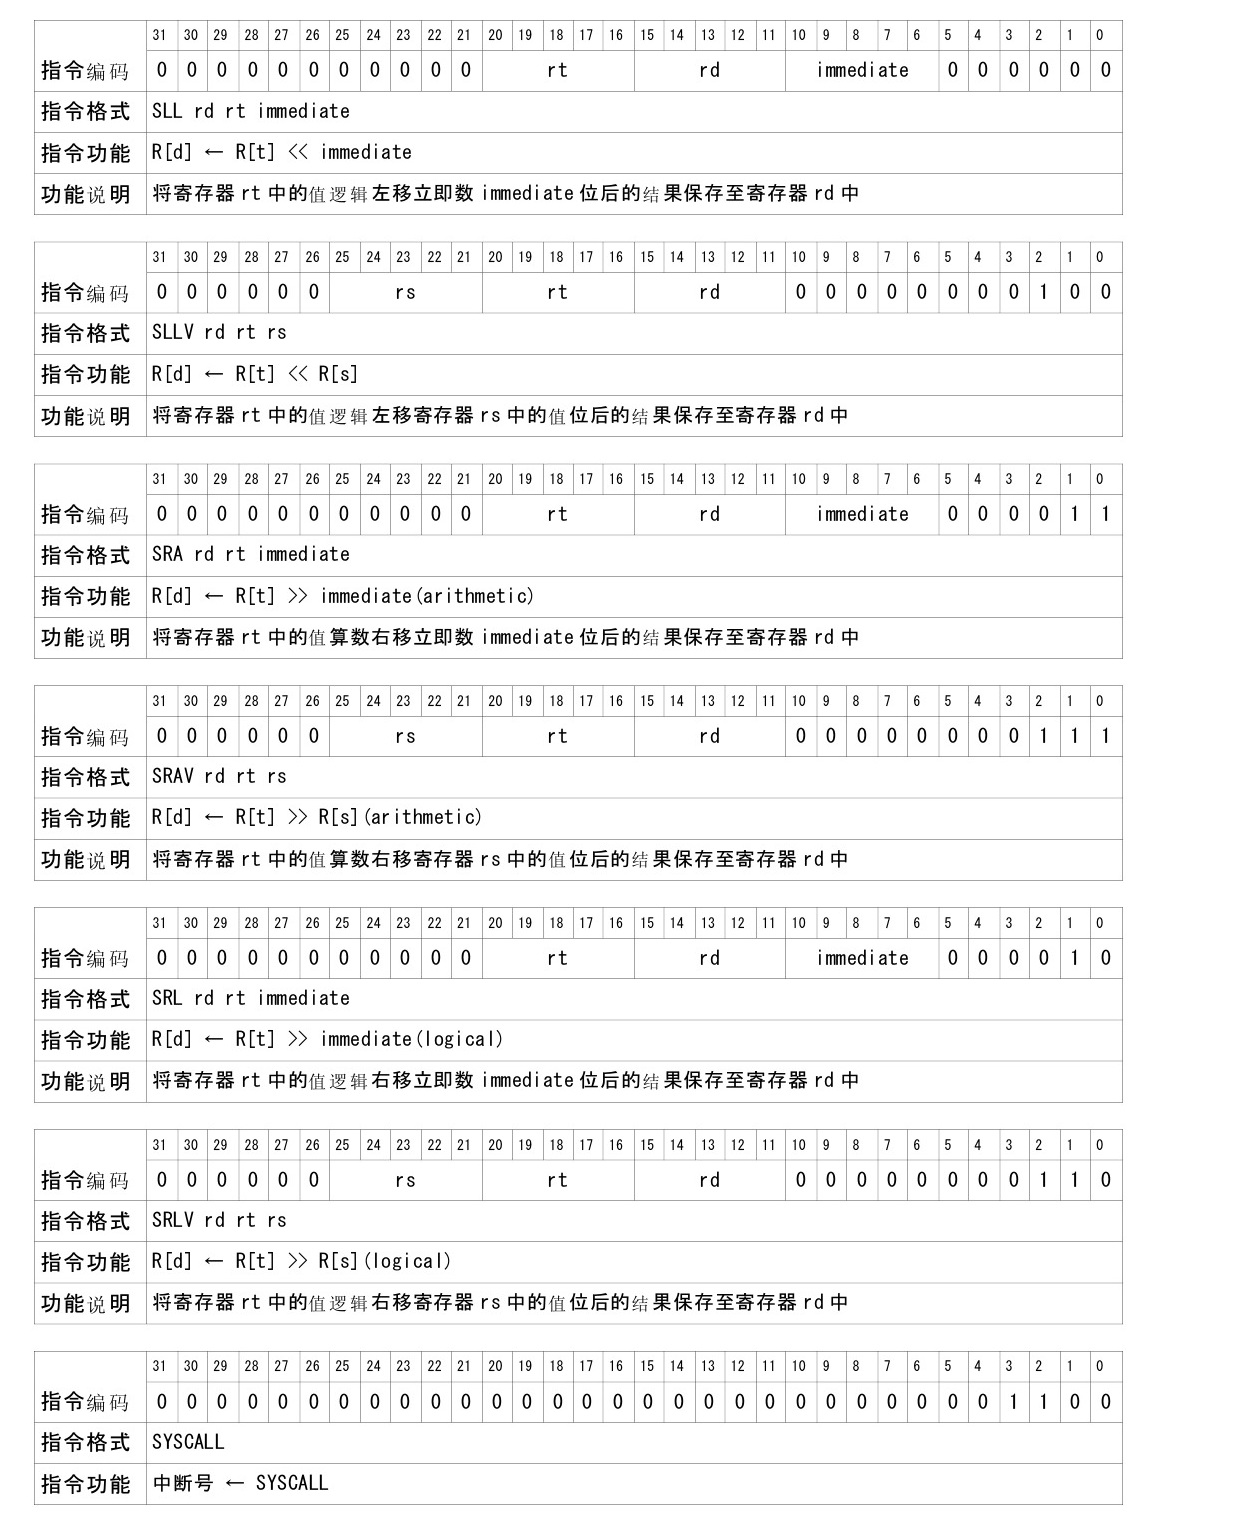
\includegraphics[width=\textwidth]{chart/insert6.jpg}
    \end{figure}

    \begin{figure}[!hbp]
            \centering
            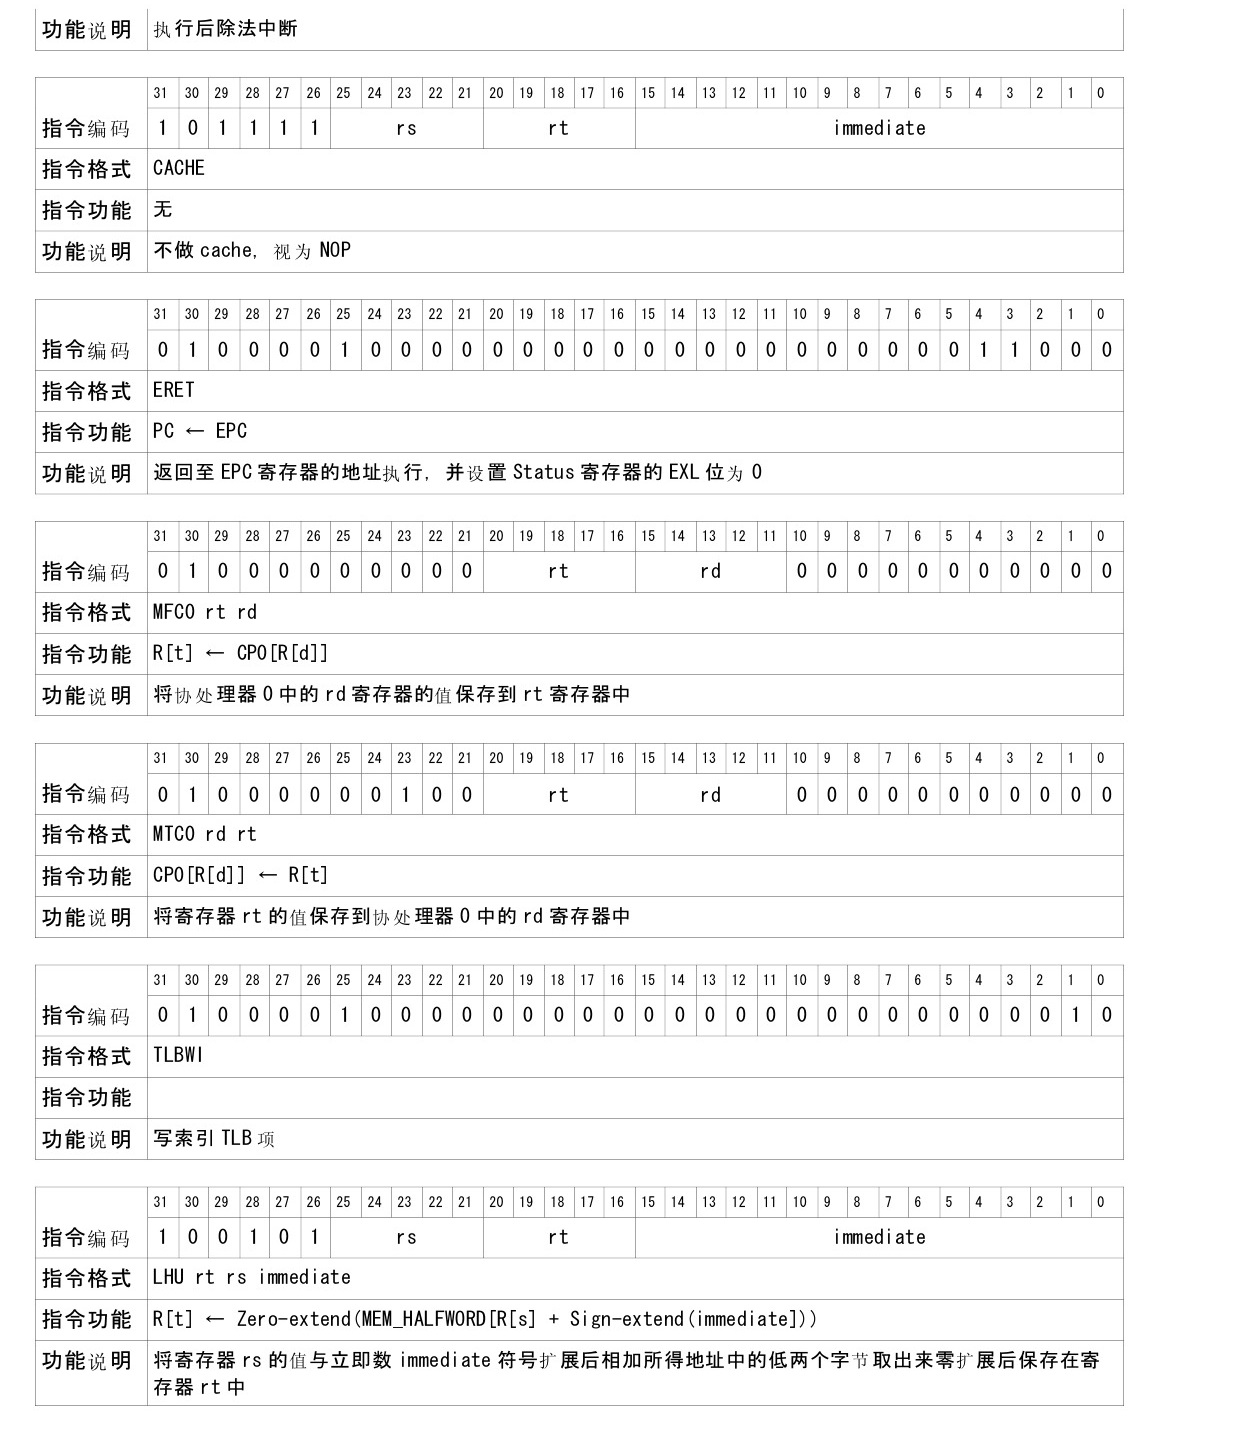
\includegraphics[width=\textwidth]{chart/insert7.jpg}
    \end{figure}
